%==================================================================================================
%   LUKES THESIS TEMPLATE 1.2
%   -------------------------
%   This template is based upon the offcial IMM PhD Thesis template, it is enhanced with a number
%   of new features and a number of errors have fixed. This template is intended to be complied to
%   PDF using PDFLATEX and is tested using the MiKTeX 2.9 LaTeX distribution.
%   It is based on the official DTU-IMM Thesis template by Finn Kuno Christensen in 2009.
%   Small bugfixes by Kasper Laursen in 2012 and 2013.
%   -------------------------
%   Last Updated: 2012-09-19
%   Contact: lthhe@imm.dtu.dk
%==================================================================================================
%
%==================================================================================================
% DOCUMENT SETUP
%==================================================================================================
\documentclass[10pt,twoside]{book}                  %Official DTU-IMM Thesis document setup
%
%Set to 'print' for printed version, use 'net' for online version
\def\thesisversion{print}
%
%==================================================================================================
% PACKAGES
%==================================================================================================
\usepackage{LukeThesis}                             %Import Thesis base style
%input{PhDMacros}                                   %Thesis specific macros
%
%==================================================================================================
% THESIS PROPERTIES (Modifiy these fields with your details)
%==================================================================================================
\def\thesisauthor{Brian Lynnerup Pedersen}          %Author
\def\thesistitle{Article Duplicates}		        %Title
\def\thesishandin{09-June}                          %Submission date (Day-Month}
\def\thesisdegree{B.Eng}                            %Degree ('B.Eng', 'B.Sc.', 'M.Sc.' or 'PhD')
\def\thesisyear{2014}                               %Submission year
\def\thesisnumber{????}                                 %DTU-IMM Serial number (do not include year)
\def\thesisISSN{0000-0000}                          %ISSN number
\def\thesiskeywords{Keywords are, comma separated}  %PDF keywords
\derivethesisprops                                  %Derive dependent properties
%
%==================================================================================================
% SECTION NUMBERING SETUP
%==================================================================================================
\setcounter{tocdepth}{2}                            %2 adds sections up to subsections
\setcounter{secnumdepth}{3}                         %Subsubsections get a number when this is 3
%
%==================================================================================================
% THESIS STRUCTURE  (Modifiy to include more chapters etc)
%==================================================================================================
\begin{document}
%------------------------
%Pre-frontmatter material
%------------------------
\prefrontmatter
%--------------------
%Frontmatter material
%--------------------
\frontmatter
\pagenumbering{roman}                               %Set frontmatter numbering style
\chapter{Summary (English)}

The goal of this thesis is to document my work with implementing a working prototype of using algorithms to find article duplicates in a large corpus of articles. I will describe how the article inflow is currently working and how Infomedia plans on implementing my work in this inflow.

I will look at various algorithms for text comparison, and look into the possibility of creating my own algorithm or tweak an existing algorithm to better suit the needs for this job.

I will do an analysis of the task, and what kind of implementation I have done.

Finally I will write a summary of the work done, problems I have come across, and what the future of the project will be.                                   %English summary of Thesis
\markboth{}{}                                       %Set headings (left)(right)
\chapter{Summary (Danish)}
\begin{otherlanguage}{danish}

Målet for denne afhandling er at dokumentere mit arbejde med at finde artikel duplikater, i et større artikel corpus, ved brug af algoritmer. Jeg vil beskrive hvordan Infomedias artikel inflow virker nu, og hvordan Infomedia planlægger at bruge mit arbejde i fremtiden.

Jeg vil undersøge forskellige tekstsammenlignings algoritmer, og undersøge muligheden for at lave min egen algoritme, eller modificere en eksisterende algoritme til at bedre udføre det arbejde jeg laver i denne opgave.

Til sidst vil jeg gennemgå det arbejde jeg har lavet, hvilke problemer jeg løb ind i og hvad fremtiden for projektet vil være.

\end{otherlanguage}                                   %Danish summary of Thesis
\markboth{}{}                                       %Set headings (left)(right)
\chapter{Preface}

This thesis was prepared at the department of Informatics and Mathematical Modelling at the Technical University of Denmark in fulfilment of the
requirements for acquiring an M.Sc. in Informatics.

The thesis deals with ...

The thesis consists of ...
%==================================================================================================
% SIGNATURE AREA
%==================================================================================================
\vspace{20mm}
\begin{center}
    \hspace{20mm} Lyngby, \thesishandin-\thesisyear
    \vspace{5mm}
    \newline
  %Update signature image file in line below
    
\includegraphics[scale=0.5]{figures/SignatureDummy}
\end{center}
\begin{flushright}
    \thesisauthor
\end{flushright}
% % % EOF % % %                                     %Preface
\markboth{}{}                                       %Set headings (left)(right)
\chapter{Acknowledgements}

I would like to thank my supervisors from DTU, Inge Li Gørtz and Philip Bille, for the help they provided to my project. Also I would like to thank my company Infomedia, for letting me do my project for them, in particular my project leader Klaus Wenzel Jørgensen and Rene Madsen.


                            %Acknowledgements
\markboth{}{}                                       %Set headings (left)(right)
%------------------
% Table of contents
%------------------
\newpage\mbox{}\newpage
\chaptermark{Contents}
\pdfbookmark{\contentsname}{toc}
\renewcommand{\sectionmark}[1]{\markright{#1}}
\sectionmark{Contents}
\addtolength{\parskip}{-\baselineskip}
\tableofcontents
\addtolength{\parskip}{\baselineskip}
\renewcommand{\sectionmark}[1]{\markright{\thesection\ #1}}
%-------------
% Main content
%-------------
\mainmatter
\chapter{Introduction}
I have been working for Infomedia\footnote{\url{www.infomedia.dk}} since my third semester at DTU, studying as an IT engineer (BSc) at DTU (march 2012). Infomedia is in \underline{short} a company that deals with news monitoring.

Infomedia is the result of a fusion between Berlingske Avisdata and Polinfo in 2002, which means that Infomedia is partly owned by JP/Politikens Hus\footnote{\url{www.jppol.dk}} and Berlingske Media\footnote{\url{www.berlingskemedia.dk}}. It is a company with around 130 employees, of which a fair amount is student aides like myself. Infomedia has various departments, which includes an economy, sales, analysis and an IT department amongst others.\\
I am employed in the IT department as a student programmer.

Infomedia deals with news monitoring, which means that we have an inflow of articles\footnote{Articles are sent to Infomedia daily, this can be more than 40,000 articles per day.} from various newspapers, news sites, television and radio media, which we then monitor for content that is of interest to our clients. This can be a client that wishes to know when their firm is mentioned in the press or a product they are using, if that is being mentioned. Infomedia have also begun monitoring social media. Infomedia then sells various solutions to clients, for them to get this news monitoring.

One of the things that Infomedia tries to do, is that we want to present our clients with a fast overview of the articles in which terms\footnote{A term is, in short, a word or a combination of words. For the rest of my thesis a term will however only be a single word.}, that trigger our news monitoring, appear. Many local newspapers are today owned by bigger media houses (like the owners of Infomedia) and as such, they will feature a lot of the articles that have also been printed in the "mother paper". This will make the same (or roughly the same\footnote{Articles can be slightly edited in order to make them fit into the layout of the various papers.}) article appear many times in news monitoring. In an effort to make the list of articles presented to the clients, easy to look at, and preventing a client having to read the "same" article many times, Infomedia has a wish to cluster article duplicates. Infomedia can then present the client with a list of articles and in that list have further sub lists that contains duplicates of the original aritcle\footnote{Or the longest article rather, as this will tend to contain the most information.}. This also have an economic factor as clients are charged per article read.

Another issue, is the issue of copyrights and when the same article will appear in different media, but without content given from the author of that article. An example that is often happening is that news telegrams from Reuters\footnote{\url{www.reuters.com}} or Ritzau\footnote{\url{www.ritzau.dk}} is published in a newspaper, but without the source indication. All news media are of course interested in knowing when their material is being published in competing media. This how ever can be tricky business, as official rules on the matter is incredible fuzzy.

I will in this thesis try and look into various ways of identifying article duplicates within a test corpus\footnote{A days worth of articles from 10/31/2013 - totalling 22.787 articles.} of articles. The long term goal for Infomedia is having this being implemented in the inflow of articles, and having a look back functionality so that we can group duplicates not just for one day, but for a longer period of time. 
						%Chapter Introduction
\chapter{General - Terms and Rules}
In the thesis a lot of terms is being used. This in concurrence with the Danish copyright laws.
\begin{itemize}
\item \textbf{Article:} For this thesis, a digital document containing the contents of a piece of news. Could originate from papers, magazines, TV or other forms of media.
\item \textbf{Corpus:} From Latin meaning \textit{body}. Describes the test set of articles being used a test set for this thesis.
\item \textbf{Term:} Basically a word. A term will be something that can be searched for.
\end{itemize}

blah about what words and terms is being used in the thesis

blah about copyright rules in Denmark...                                  %Chapter 1
\chapter{General - Terms and Rules}

I will in this chapter cover the essentials of the expressions and terms used throughout this thesis.

\section{Terms}

As there is a lot of terms used in this thesis, a short introduction to the most used are in order.
\begin{itemize}
\item \textbf{Article:} For this thesis, a digital document containing the contents of a piece of news. Could originate from papers, magazines, TV or other forms of media. For this thesis a document corresponds to an article. Articles are in their electronic form stored at Infomedia as XML files, I will throughout this thesis only deal with the part of the XML files that contains data of value to me in this assignment. This being \textit{Tags} (see below), \textit{Headline}, \textit{Sub headline} and \textit{Article Text}.
\item \textbf{Corpus:} From Latin meaning \textit{body}. In this thesis that describes the test set of articles being used a test set throughout my thesis.
\item \textbf{Monitoring:} In relation to the news monitoring (news surveillance) that Infomedia does, is the act of collecting news that holds information of value to our customers.
\item \textbf{Tag:} Used in Ontology\footnote{\url{http://en.wikipedia.org/wiki/Ontology_(information_science)}} to create words that describes the contents of an article.
\item \textbf{Term:} Basically a word. A term will be something that can be searched for.
\end{itemize}

\section{Matching}
I will in this thesis talk about false and true positives and negatives. A match will mean that two articles to some extend have the same content.

\begin{itemize}
\item \textbf{False Positive:} When an algorithm wrongfully identifies two articles as a match.
\item \textbf{False Negative:} When an algorithm wrongfully identifies two articles as not being a match, when in fact they are a match.
\item \textbf{True Positive:} When an algorithm correctly identifies two articles as a match.
\item \textbf{True Negative:} When an algorithm correctly identifies two articles as not being a match.
\end{itemize}


\section{Duplicates}
In this thesis I will often use the term 'duplicates' or 'match' about article comparisons. A duplication (match) can be an article that has been taken directly from a news feed and posted in a newspaper. Many local newspapers is owned by larger newspapers, and they will often receive articles from their owning paper. They will then print this in their own paper. Sometimes they will only use parts of the article and this will also be considered a duplicate for this thesis. As such duplication in this thesis is a way of describing how similar two articles are, rather than saying different papers are doing conscious fraud. That is a matter for another thesis.

\subsection{Topic Matching}
When looking at article matching, there is also the possibility of having articles score pretty well by the algorithms because they are dealing with the same topic. There are cases where the article have been heavily modified, and then there would be no basis to talk about duplication, then one could talk about topic matching. The article no longer contains the same phrases, but deals with the same topic.
Of course two articles could describe the same topic, but never have been related to begin with. I will not try and dissect whether this is the case, only try and indicate when I find two articles that are dealing with the same topic, and mark them as such. 

\subsection{Copyright}
It is hard to talking about duplicating without talking about copyrights. Although this thesis will not delve into whether something is duplicated as a part of a copyright infringement, it seems only reasonable to give a moment to talk about what a copyright is, and how it would affect duplication.

I feel that this quote is fulfilling as to explaining the concept of \textit{'copyright'}, even if it is talking about a case that is ongoing in USA at the time, and copyright rules can vary from nation to nation.
\begin{quote}
A copyright is basically a legal protection for an original expression on a fixed medium. So a song on a record, words on a page, ballet steps written down, and paint on a canvas are all copyrightable things. A phone book is not copyrightable (it’s not original). A copyright only protects the expression and not the underlying idea. Marvel does not have a corner on men in mechanical suits who fight crime – they only have the particular expression of that idea in Iron Man comic books.

Confused? That's okay. Copyrights are pretty complex things. A lot of what can be copyrighted is figured out in court when people fight over it. The basic test that the court will pose in this case is “is the expression original? Does the potentially infringing work actually borrow from the original expression?” ~\cite{Copyright}
\end{quote}

So the whole concept is extremely fuzzy, and often the infringement part will have to be settled in court. In the recent years that have been a lot of debate in which university educated people have become accused of plagiarism  in relation to their doctoral or master thesis\footnote{\url{http://www.theguardian.com/world/2011/feb/16/german-defence-minister-plagiarism-accusation}}$^{,}$\footnote{\url{http://www.nytimes.com/2012/04/03/world/europe/hungarian-president-pal-schmitt-resigns-amid-plagiarism-scandal.html?_r=0}}. A hard topic to deal with in a fixed way, and to top it off, there is also the notion of \textit{"fair use"}\footnote{\url{http://www.umuc.edu/library/libhow/copyright.cfm\#fairuse_definition}}. Although there is no real fair use paragraph in Danish law, we instead have \textit{'låneregler'}\footnote{\url{http://da.wikipedia.org/wiki/Fair_use}}. 

In the world that Infomedia is dealing with, articles are also a target of duplication, and a lot of effort have begun being invested into this, as it can be a question about a lot of money if you fail to protect your copyrighted material. So the motivation in finding article duplicates can be two sided. First off, it creates a better overview for Infomedia's customers, secondly newspapers are very interested in finding out if their material is being used, unlicensed, in other media.




Hvornår er en artikel et duplikat (korte artikler (breaking news), hvornår er to artikler "tilstrækkeligt" forskellige?)
blah about copyright rules in Denmark...                                 %Chapter 2
\appendix
\chapter{Test Diagrams}

Examples of comparing two articles with LCS. More files can be found in the electronic appendixes.

\begin{sidewaysfigure}
	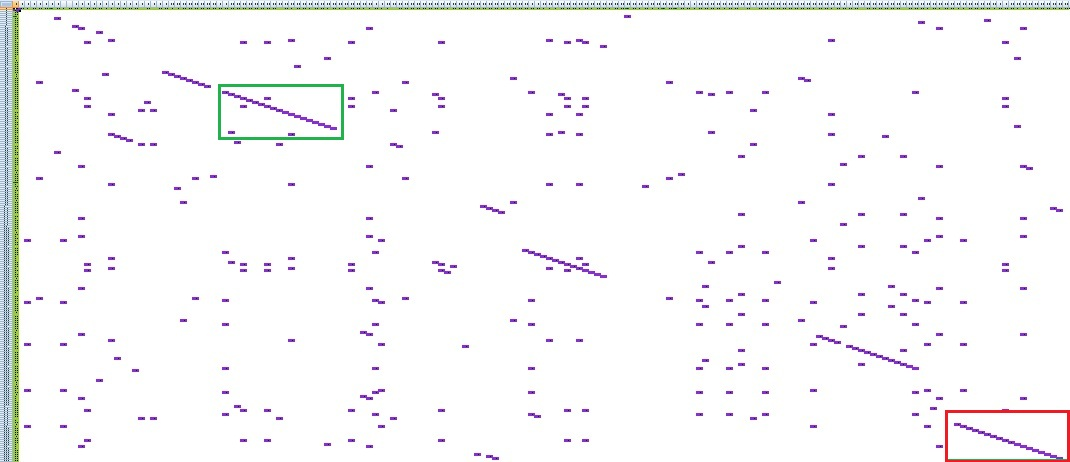
\includegraphics[scale=0.65]{figures/LcsExample}
	\caption{Diagram showing the result of two article being compared by using LCS.}
\end{sidewaysfigure}

\begin{sidewaysfigure}
	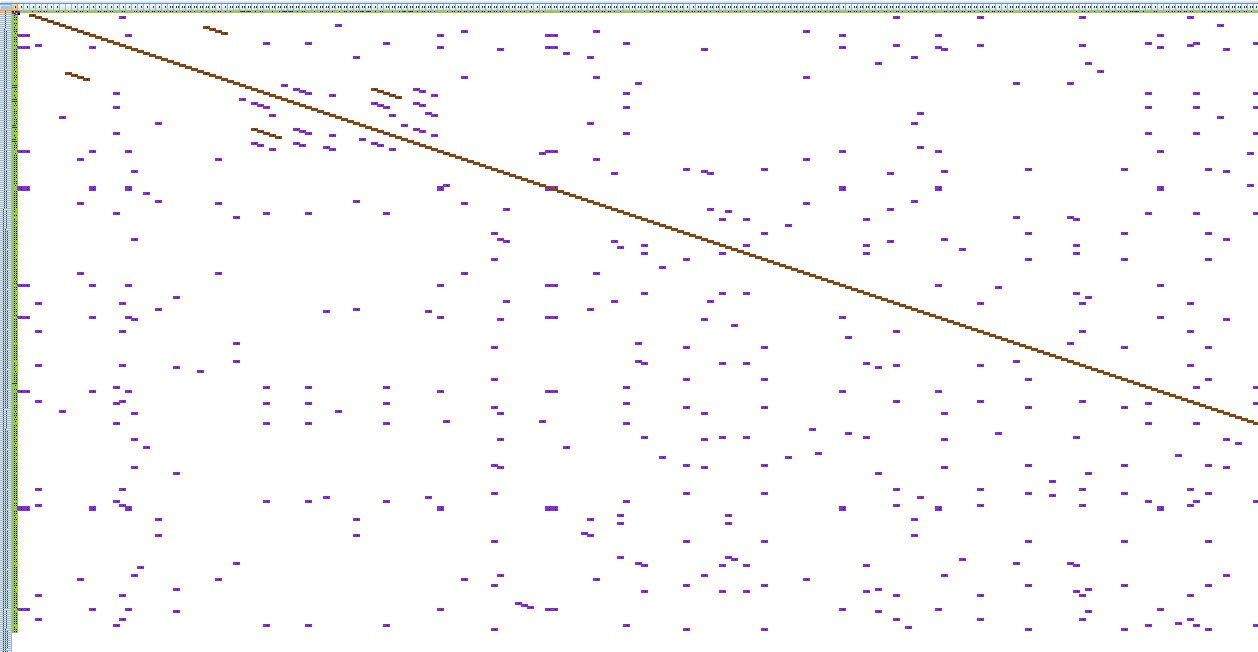
\includegraphics[scale=0.5]{figures/PerfectMatch}
	\caption{Diagram showing part of the result from running LCS on two articles that are almost a perfect match.}
\end{sidewaysfigure}

\begin{sidewaysfigure}
	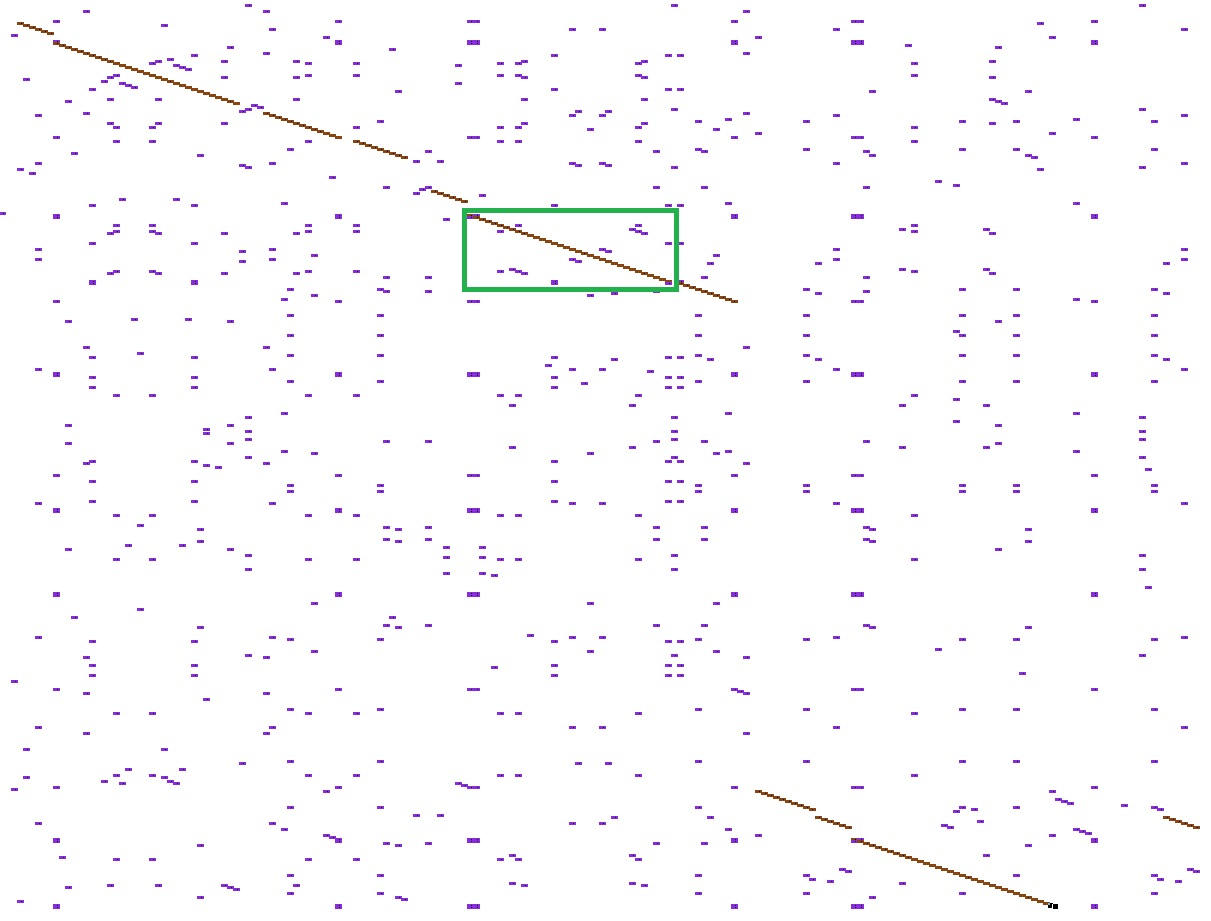
\includegraphics[scale=0.5]{figures/SubstringCollection}
	\caption{Diagram showing part of the result of running LCS on two articles and marking up all substrings with a length larger than three words.}
	\end{sidewaysfigure}                                 %Appendix A
%-----------
% Backmatter
%-----------
\backmatter
\chaptermark{Bibliography}
\renewcommand{\sectionmark}[1]{\markright{#1}}
\sectionmark{Bibliography}
\addcontentsline{toc}{chapter}{Bibliography}        %Force addition of Bibliography to TOC
\bibliographystyle{alpha}                           %Use alpha codes for references
\bibliography{References}                           %Bibliography file called
\end{document}
% % % EOF % % %